\def\pgfsysdriver{pgfsys-dvipdfm.def}
\documentclass{beamer}

%\usetheme{Madrid}

\usepackage{color}
\usepackage{xcolor}
\usepackage{indentfirst}
\usepackage[export]{adjustbox}
\usepackage{float}
\usepackage{wrapfig}
\usepackage{setspace}
\usepackage{fontspec}
\usepackage{graphicx}
\usepackage{subcaption}
\usepackage{pgfpages}
\setbeameroption{show notes}
\setbeameroption{show notes on second screen=right}
%\setbeamertemplate{note page}[plain]
\setbeamertemplate{note page}{\vspace{10pt}\insertnote}

\setbeamertemplate{footline}{}
\setbeamertemplate{navigation symbols}{}

\setmainfont{Open Sans}
\setsansfont{Open Sans}

\setbeamerfont{framesubtitle}{size={\fontsize{11}{11}}}
\setbeamerfont{note page}{size={\fontsize{12}{14}}}
%\setbeamerfont{framesubtitle}{size=\Large}


\setbeamertemplate{itemize items}[ball]

\title{Merits of Online Education}
%\title{Merits of Selective Education}
\author{Huan Li}

\begin{document}
\begin{spacing}{1.2}

\frame{\titlepage}
\note{
{\color{red} (12s) Okay, so today I'm gonna talk about the topic of online education. And here my argument is that the online education is better than the traditional classroom education, so I'm gonna focus more \boxed{on\ its} merits.}
}

\begin{frame}
	\frametitle{Massive Open Online Course (MOOC)}
	
	%\begin{wrapfigure}{R}{0.2\textwidth}
	%	\centering
	%	
\includegraphics[width=0.25\textwidth]{mooc.eps}
	%\end{wrapfigure}
	%\vspace{-9.5pt}
	\begin{figure}
		%\centering
		%
\includegraphics[width=0.6\textwidth]{mooc.eps}
		\makebox[\linewidth][c]{
		\begin{subfigure}[H]{0.48\textwidth}
			%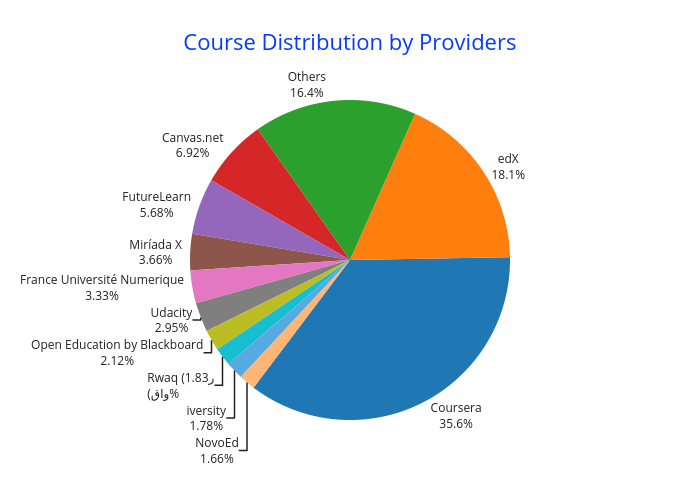
\includegraphics[width=1\textwidth]{mooc_providers2.png}
			
\includegraphics[width=1\textwidth]{mooc.png}
		\end{subfigure}
		\quad
		\begin{subfigure}[H]{0.52\textwidth}
			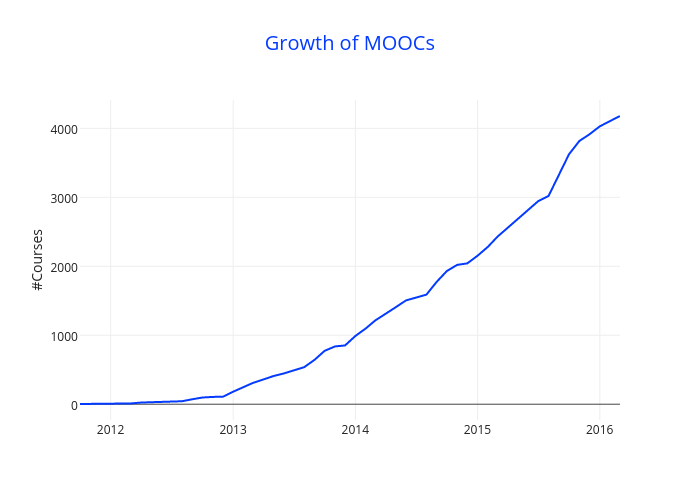
\includegraphics[width=1\textwidth]{mooc_growth2.png}
		\end{subfigure}
		}
	\end{figure}
	
	MOOC
	\begin{itemize}
		%\item Merits of MOOC
		%\begin{itemize}
			\item Reduces the cost of education
			\item Broadens access to education
			\item Leads to better academic performance
		%\end{itemize}
	\end{itemize}
\end{frame}
\note{
	%Since 2012, several course providers have emerged, and provided massive open online courses, which are also known as MOOCS.
	
	
	(41s) In the last few years, there has been a great proliferation in MOOCs, which are also known as massive open online courses.
	
	
	
	{\color{blue} These courses are provided by several different platforms, such as edX, Coursera and Udacity. They offer all kinds of courses from top universities like Standford and MIT.} %Some of them are for-profit as Coursera and Udacity, while others are non-profit as edX.}
	
	{\color{orange} So that these university subjects become available and free of charge to anyone on the internet. } %
%They offer all kinds of courses from top universities like Standford and MIT. }
	
	%{\color{Mulberry} Many course providers offer various kinds of courses. For example, edX offers courses from Universities like Harvard and MIT, Udacity offers courses for sciences, and }
	 
	%{\color{orange} MOOCs are mostly offered by universities, like Coursera and edX by Stanford and MIT. But they can also come from other organizations, such as British Library in Future Learn. }
	
	{\color{red} Currently, there are 3 major merits of MOOCs. That is, it cuts down the \boxed{cost\ of} education, it broadens access to education, and it leads to better academic performance. }
	 
%	MOOCs platforms can either be specilized, such as Udacity for sciences, or provide a wide range of subjects, like Coursera.


	
}

\begin{frame}
	\frametitle{Reduction in the Cost of Education}
	\framesubtitle{Virtual classrooms}
	\begin{figure}
		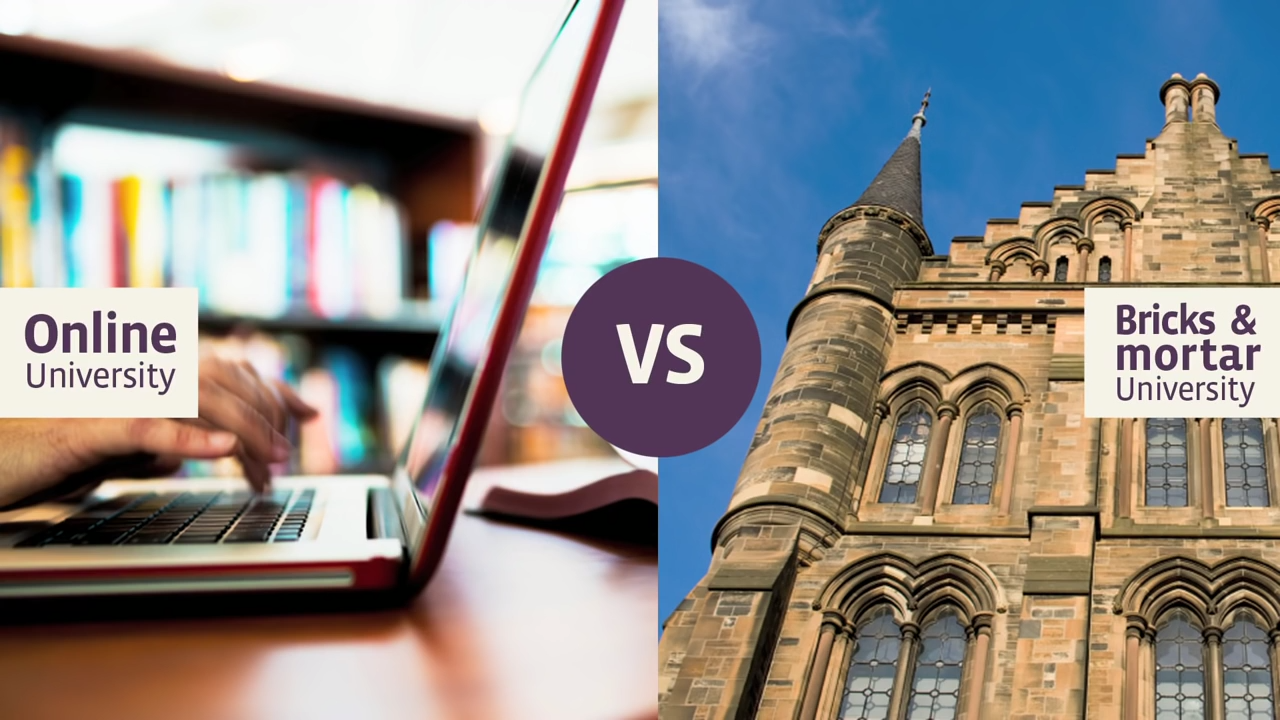
\includegraphics[width=1\textwidth]{low_cost_1.png}
	\end{figure}
\end{frame}
\note{
	{First of all, when it comes to online education, there's no need for classrooms or seats in'em. So the expense can be saved, and won't be passed to students any more. Also there's no need to worry about capacity of classrooms, \boxed{because} there are no limits of seats in virtual university.}
}

\begin{frame}
	\frametitle{Reduction in the Cost of Education}
	\framesubtitle{Open Educational Resources (ORE)}
	\begin{figure}
		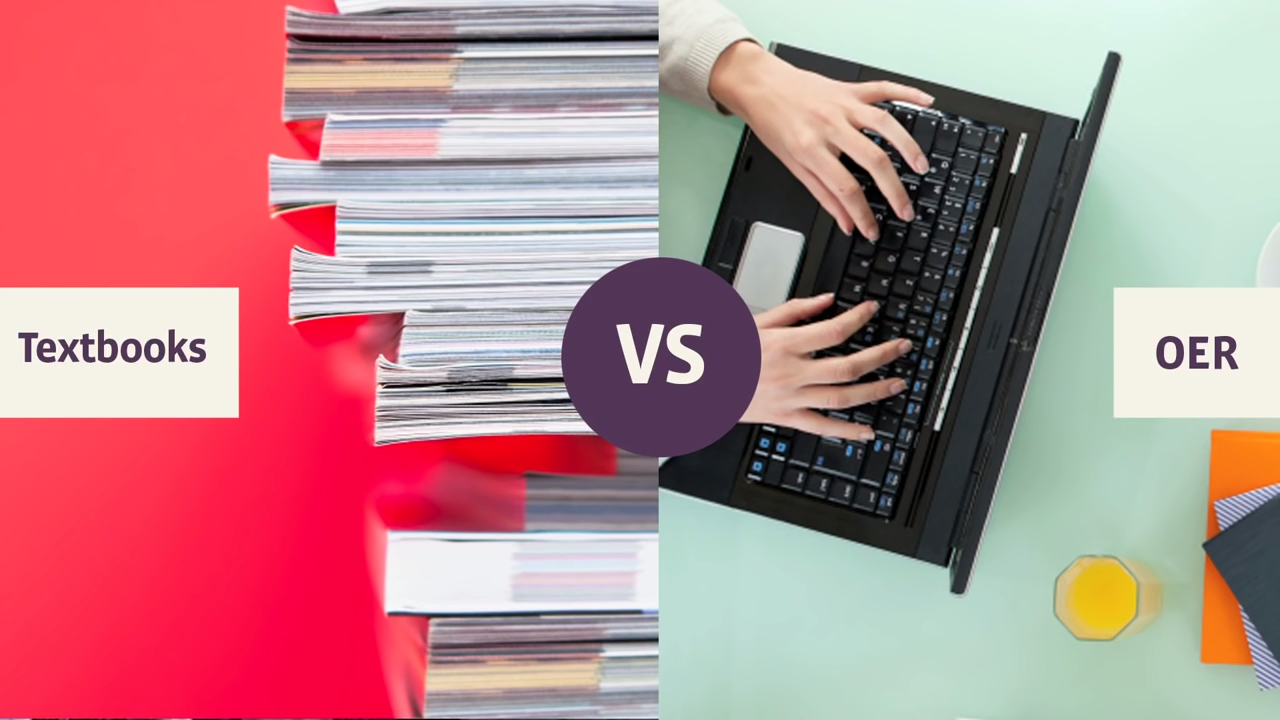
\includegraphics[width=1\textwidth]{low_cost_2.png}
	\end{figure}
\end{frame}

\note{
	{\color{blue} And moreover, textbooks are free to students. By using open educational resources, or some other free material offered by professors, students don't have to buy textbooks, which are usually at very high prices.}
}
\begin{frame}
	\frametitle{Reduction in the Cost of Education}
	\framesubtitle{Peer-to-peer Learning}
	\begin{figure}
		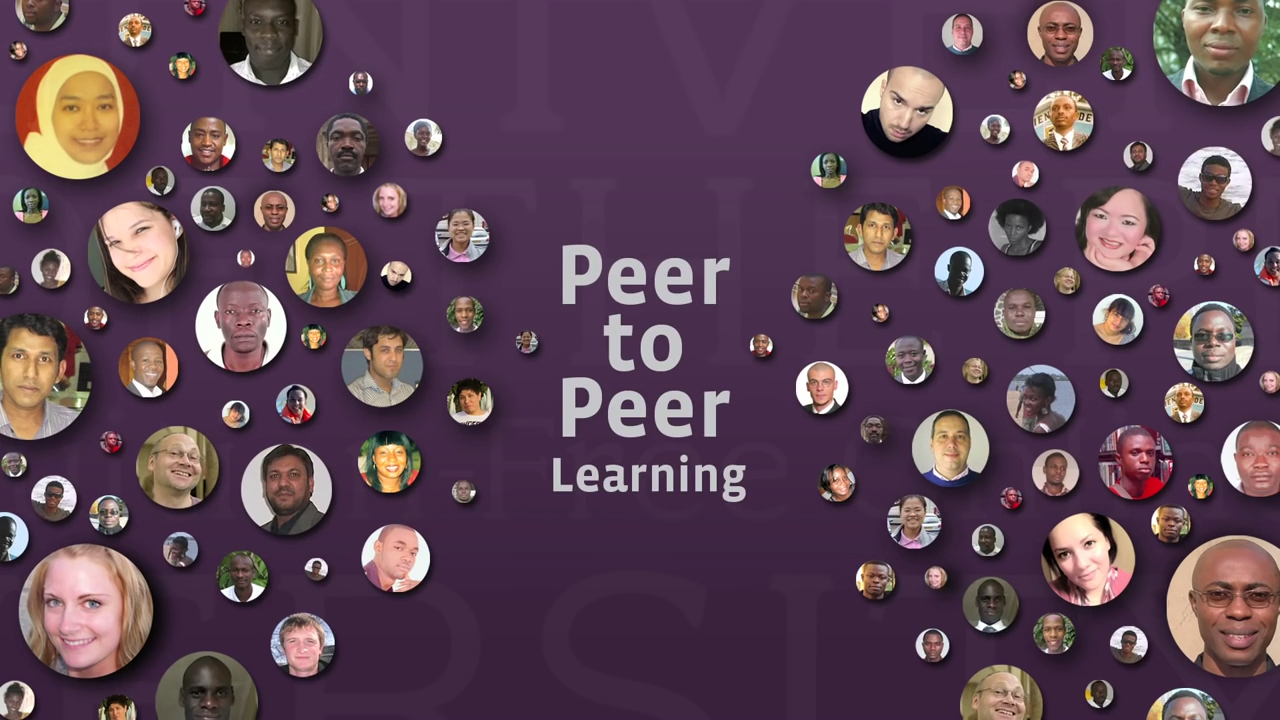
\includegraphics[width=1\textwidth]{peer-to-peer.png}
	\end{figure}
\end{frame}

\note{
	{\color{red} Finally, peer-to-peer learning can be applied in online education. Students from all over the world can interact and study together. They can even grade each other's homework. So that professors don't need to grade all the assignments by themselves, which can save'm a lot of time.
}
}

\iffalse
\begin{frame}
	\frametitle{Reduction in the Cost of Education}
	
	\begin{figure}
		\makebox[\linewidth][c]{
		\begin{subfigure}[H]{0.5\textwidth}
			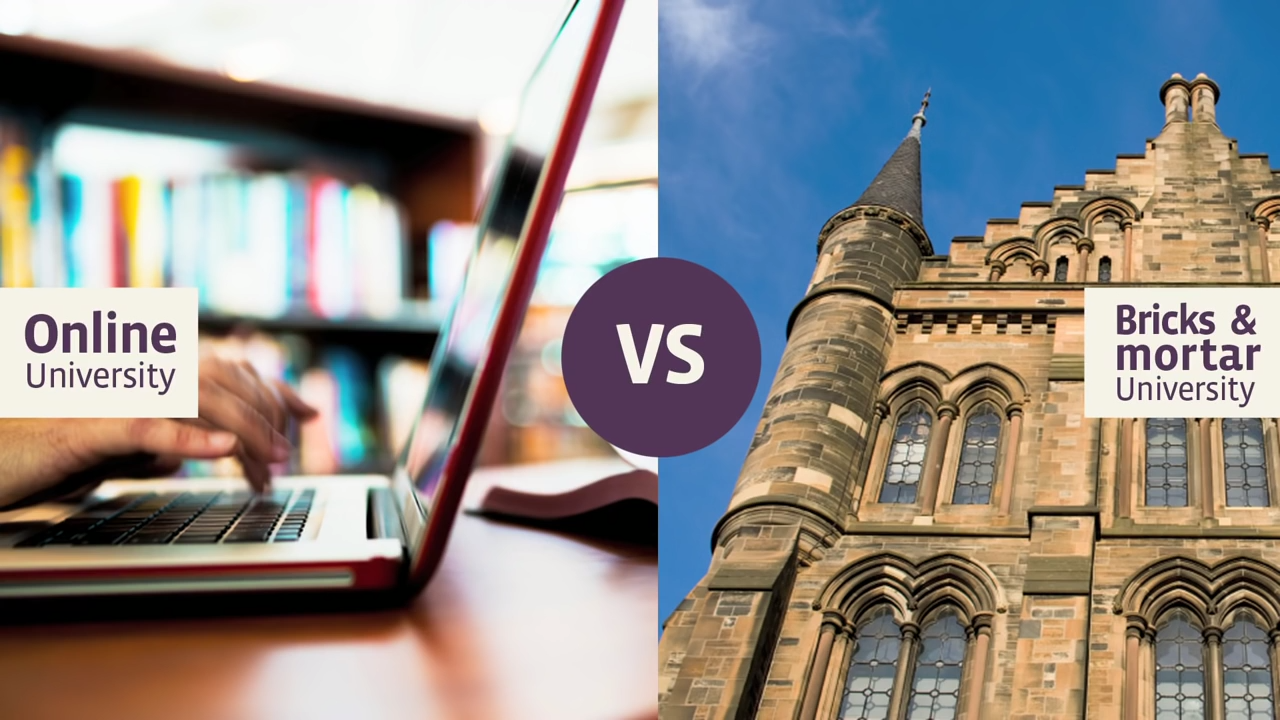
\includegraphics[width=1\textwidth]{low_cost_1.png}
		\end{subfigure}
		\hspace{-5.75pt}
		%\quad
		\begin{subfigure}[H]{0.5\textwidth}
			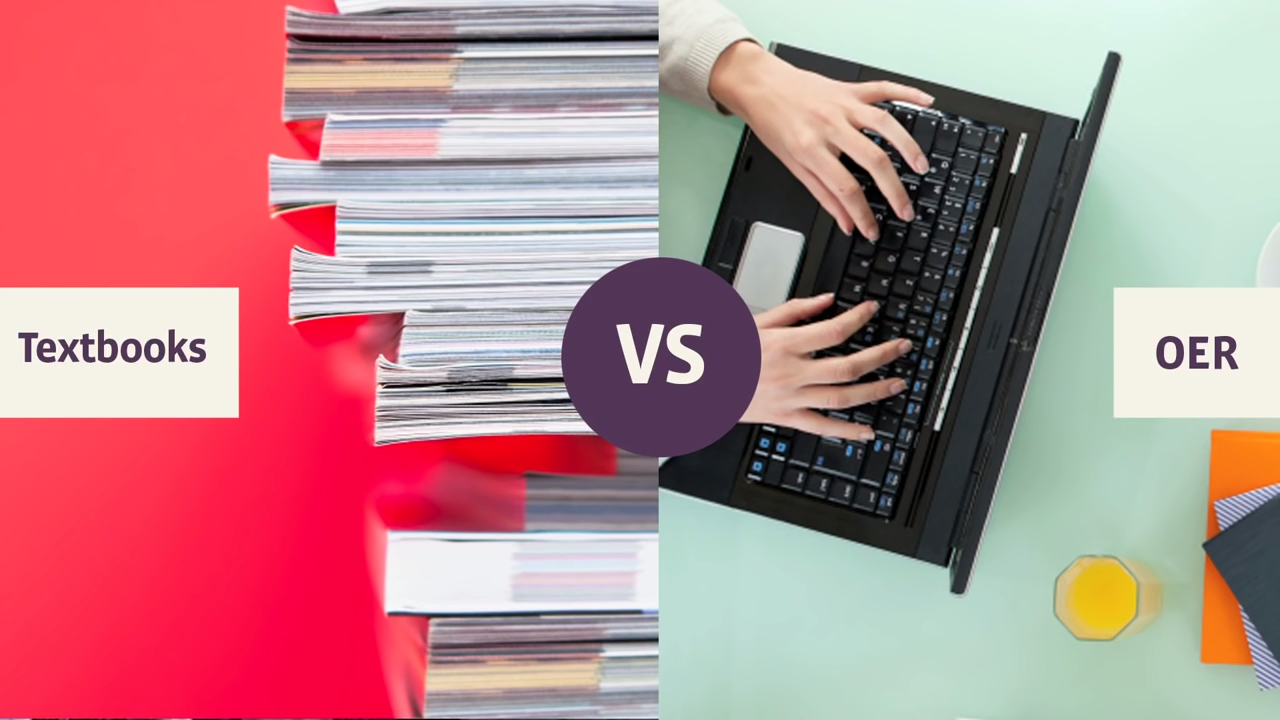
\includegraphics[width=1\textwidth]{low_cost_2.png}
		\end{subfigure}
		}
	\end{figure}
	
	\begin{wrapfigure}{R}{0.5\textwidth}
		\vspace{-16.9pt}
		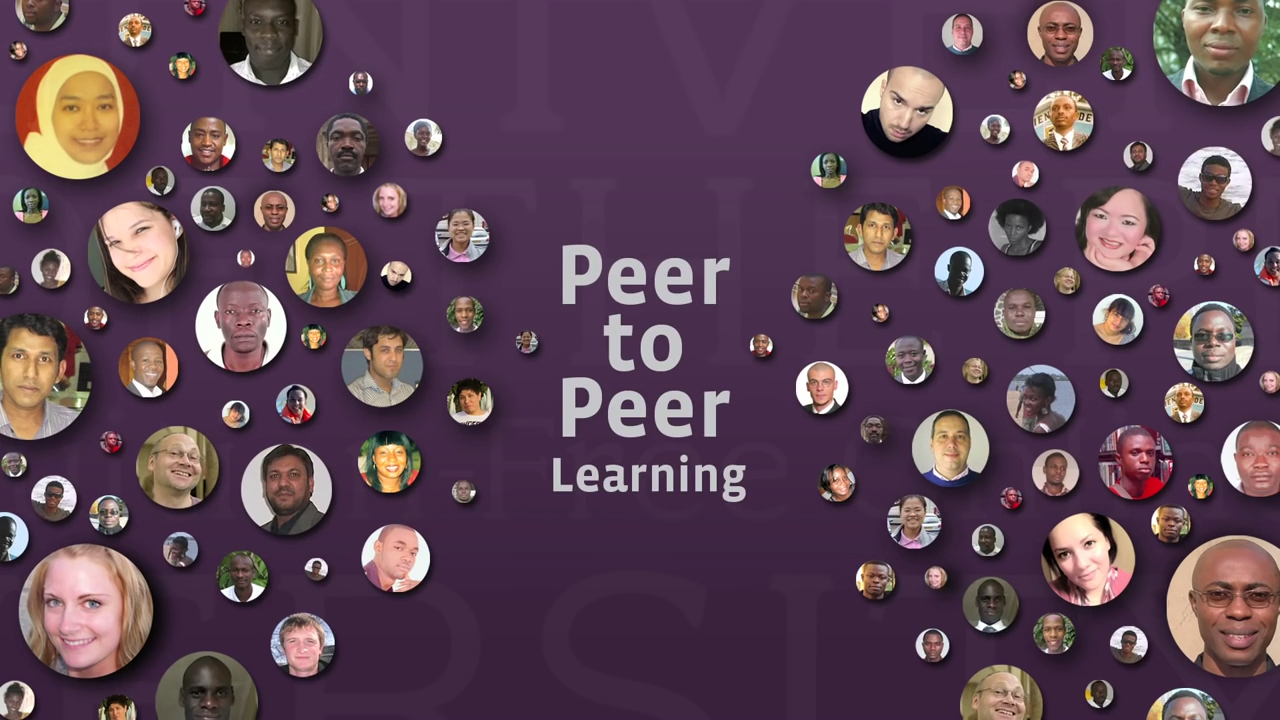
\includegraphics[width=0.5\textwidth]{peer-to-peer.png}
	\end{wrapfigure}
	\
	\begin{itemize}
		\item Virtual classrooms
		\item Open educational resources
		\item Peer-to-peer learning
	\end{itemize}
	
\end{frame}
\note{
	(42s) First of all, when it comes to online education, there's no need for classrooms or seats. So the expense can be saved, and won't be passed to students.	Also there's no need to worry about capacity of classrooms, because there are no limits of seats in virtual university.
	
	{\color{blue} Also, Textbooks are free to students. By using open educational resources, students don't have to buy textbooks at high prices.}
	
	{\color{red} Finally, peer-to-peer learning can be applied in online education. Students from all over the world can interact and study together. They can even grade each other's homework. So that it can reduce the time that professors need to assess assignments.
}
}
\fi

\begin{frame}
	\frametitle{Broad Access to Education}
	%\vspace{-9pt}
	\begin{figure}
		%\centering
		%
\includegraphics[width=0.6\textwidth]{mooc.eps}
		\makebox[\linewidth][c]{
		\begin{subfigure}[H]{0.48\textwidth}
			%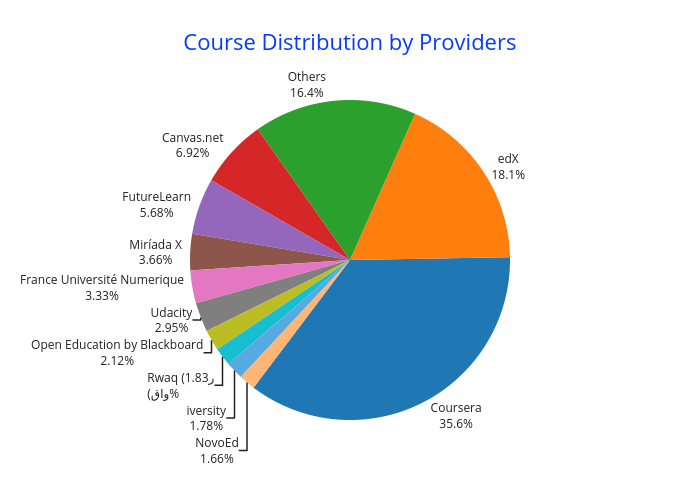
\includegraphics[width=1\textwidth]{mooc_providers2.png}
			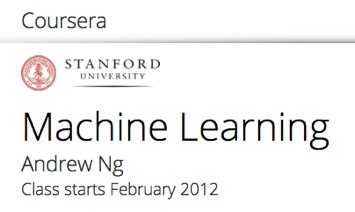
\includegraphics[width=1\textwidth]{machine_learning.jpg}
		\end{subfigure}
		\quad
		\begin{subfigure}[H]{0.48\textwidth}
			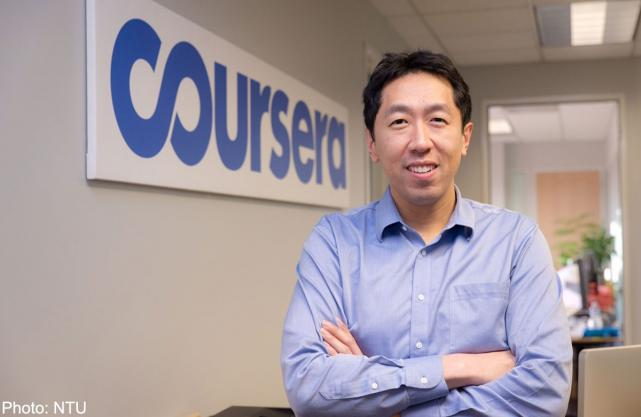
\includegraphics[width=1\textwidth]{andrew_coursera.jpg}
		\end{subfigure}
		}
	\end{figure}
	%\begin{figure}[H]
	%	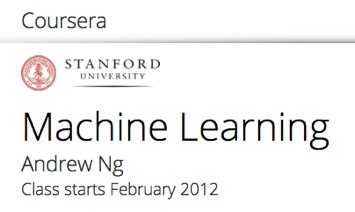
\includegraphics[width=0.55\textwidth,left]{machine_learning.jpg}
	%\end{figure}
	%\begin{wrapfigure}{R}{0.5\textwidth}
	%	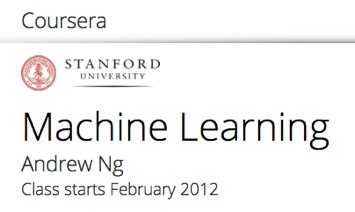
\includegraphics[width=0.5\textwidth]{machine_learning.jpg}
	%\end{wrapfigure}
	The Machine Learning class offered by Andrew Ng:
	\begin{itemize}
		%\item one of the biggest classes in Stanford
		\item 400 people enrolled every time it's offered
		\item 100,000 people registered when it's taught to the public%Andrew taught the class to the general public
	\end{itemize}
	Hence, Andrew and his colleague formed Coursera.
	%{\small
	%\noindent The machine learning class offered by Andrew Ng is one of the biggest classes in Stanford. It has 400 people enrolled every time it's offered. When Andrew taught the Machine Learning class to the general public, it had 100,000 people registered. So to put that number in perspective, for Andrew to reach that same size audience by teaching a Stanford class, he would have to do that for 250 years.}
\end{frame}
\note{
	(43s) Because MOOCs can be accessed by anyone on the internet, it makes education more available than ever before. 
	
	{\color{blue} Let's take the Machine Learning class by Andrew Ng for example.}
	
	{\color{orange} Every time the course was offered in Stanford, about 400 students would enroll. And this already makes the Machine Learning course one of the biggest in Stanford. But when Andrew taught this course to the public for the first time, about 100 thousand people registered for it, which is nearly 250 times more}
	
	{\color{red} So, having seen the impact of this, Andrew and his colleague decided that they needed to scale this up. So they formed Corsera, to bring top-quality education to as many people as they could.}
}

\begin{frame}
	\frametitle{Better Academic Performance}
	%\vspace{-9.5pt}
	\begin{figure}
		\includegraphics[width=\textwidth]{San_Jose.png}
	\end{figure}
	%\quad
	Key ideas: active learning, self-pacing, and instant feedback.
%Key ideas that make all of this work:
	%\begin{itemize}
	%	\item Active learning
	%	\item Self-pacing
	%	\item Instant feedback
	%\end{itemize}
\end{frame}
\note{
	(44s) And it also turns out, MOOCs can lead to better academic performance. 
	
	{\color{blue} There was once a pilot course in San Jose State University. It was s a hard course about circuits and electronics. The course was designed to be a blended one. That is, the students first watched videos and did interactive exercise online, and then they came to classrooms to discuss with classmates and professors.}
	
	{\color{orange} As it was a hard course, the failure rate of it used to be about 40 to 41 percent. But with this blended class, the failure rate fell to 9 percent. So the result was extremely good.}
	
	{\color{red} And speaking of the reasons for this, there are three key ideas that make all of this work.}
}

\begin{frame}
	\frametitle{Better Academic Performance}
	\framesubtitle{Active Learning}
	{\tiny [1] Craik, F.I. and Lockhart, R.S., 1972. Levels of processing: A framework for memory research.\\ \textit{Journal of verbal learning and verbal behavior}, 11(6), pp.671-684.}
	\vspace{-5pt}
	\begin{figure}[H]
		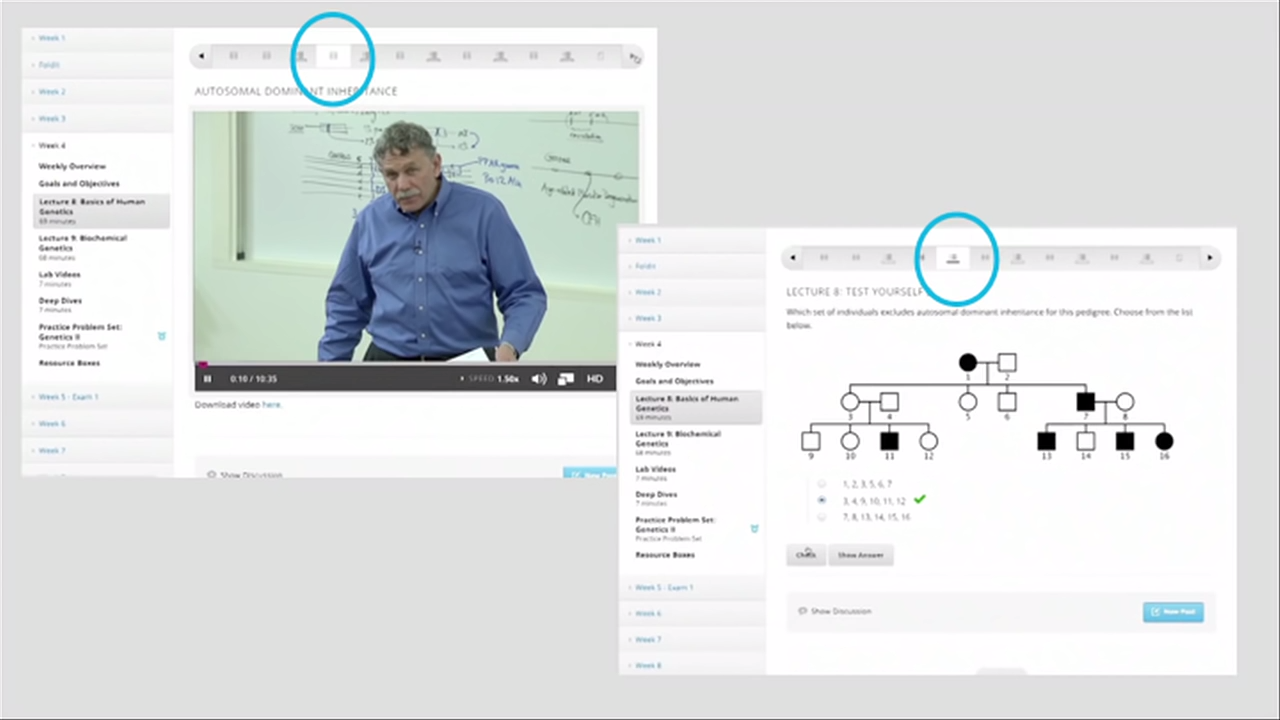
\includegraphics[width=\textwidth]{active_learning.png}
	\end{figure}
	%\vspace{-15pt}
	
\end{frame}
\note{
	(23s) The first one is active learning. 
	\vspace{10pt}
	
	{\color{blue} Each lesson of this course is a sequence of videos and interactive exercise. So a student may watch a five- or seven-minute video and follow that with an interactive exercise. }
	\vspace{10pt}
	
	{\color{red} This form of learning is called active learning. And according to the research, students learn much better when they are interacting with the material in this way.}
}

\begin{frame}
	\frametitle{Better Academic Performance}
	\framesubtitle{Self-pacing}
	\begin{figure}
		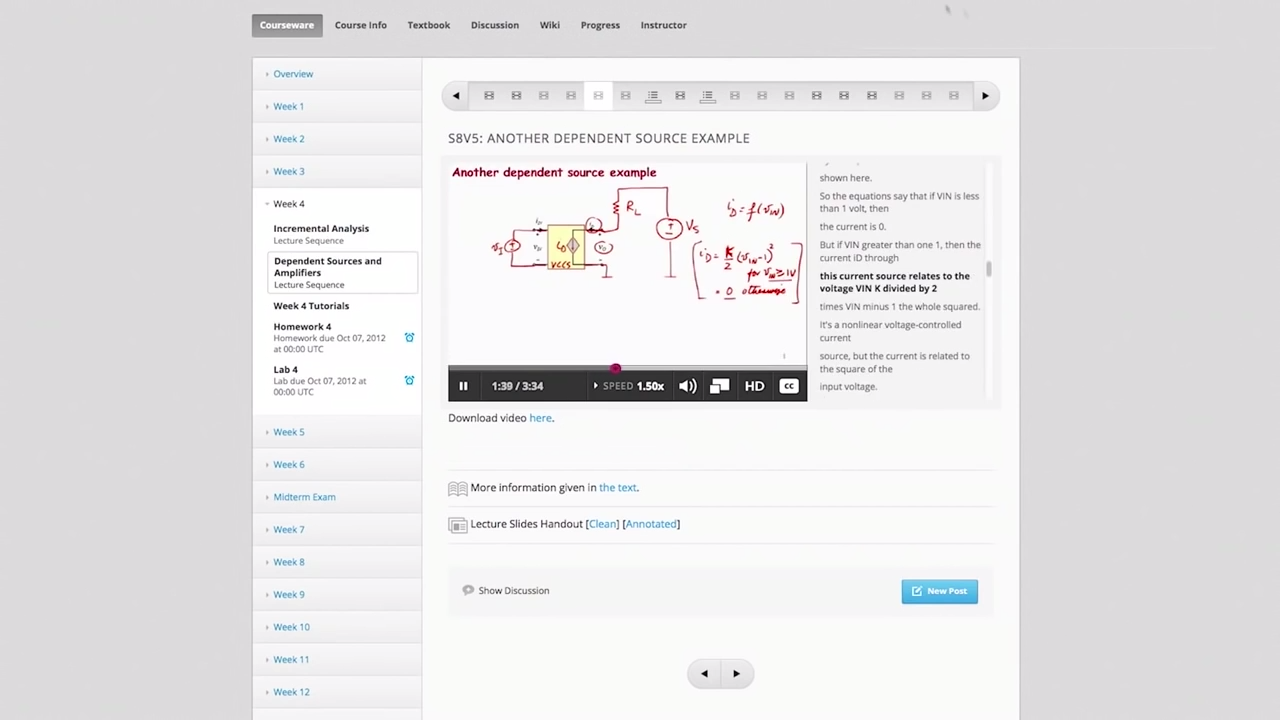
\includegraphics[width=\textwidth]{self-pacing.png}
	\end{figure}
\end{frame}
\note{
	(27s) The second idea is self-pacing.
	\vspace{10pt}
	
	{\color{blue} When having classes in classrooms, students may not be concentrated all the time. For example when they are taking notes, they may lose the professor. And if the class is a hard one, they may even lose the lecture for the rest of the hour.}
	\vspace{10pt}
	
	{\color{red} But when they are watching video lectures, they can pause the video when they're taking notes. Or they can even rewind the professor in case they don't understand. So this form of self-pacing can be very helpful to learning.}
}

\begin{frame}
	\frametitle{Better Academic Performance}
	\framesubtitle{Instant Feedback}
	\begin{figure}
		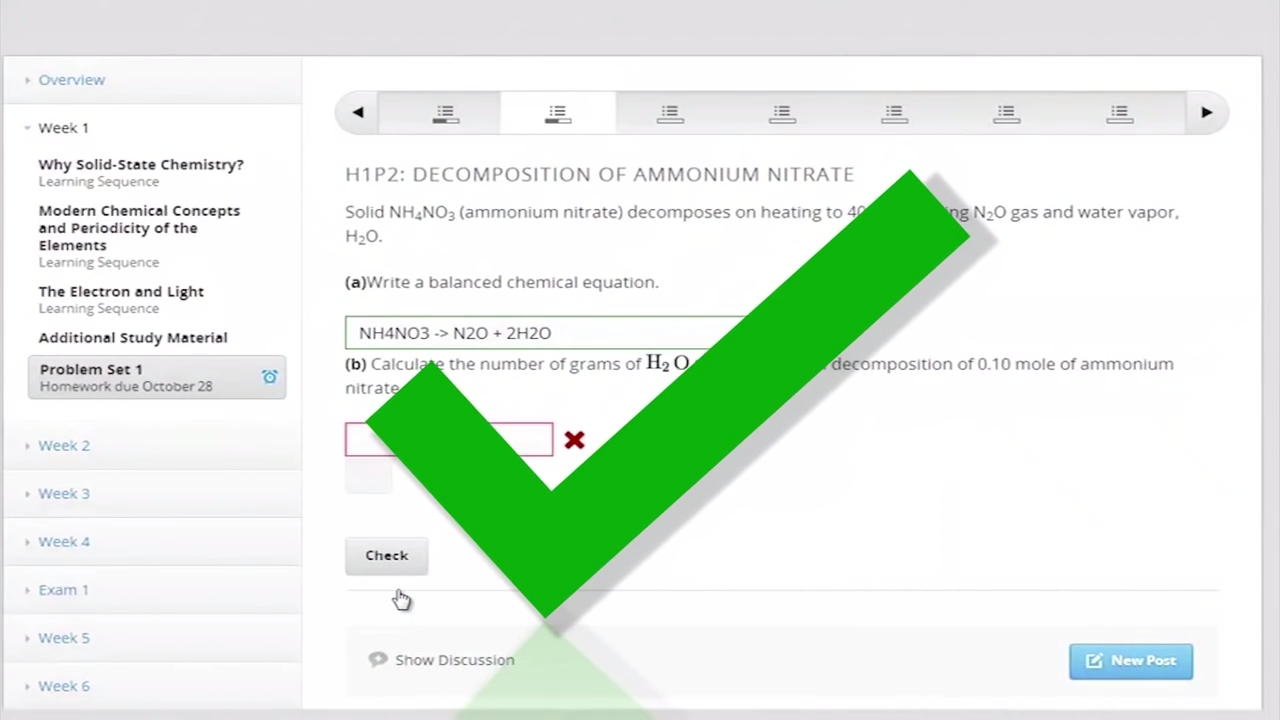
\includegraphics[width=\textwidth]{instant_feedback.png}
	\end{figure}
\end{frame}
\note{
	(33s) The third idea is instant feedback.
	\vspace{10pt}
	
	{\color{blue} In traditional classroom courses, it takes a really long time to grade all of the homework. Students may have forgotten all about it when their grades come back. And some of the homework may be not even graded ever.}
	\vspace{10pt}
	
	{\color{red} But with instant feedback, the computer grades all of the assignments. So students can try to apply their answers. If they get it wrong, they can get feedback at once. So that they can try it over and over again before they find the right answer. This would make the learning process much more engaging, and hence make students learn it better. }
}

\begin{frame}
	\frametitle{Conclusions}
	\vspace{-13pt}
	\begin{figure}
		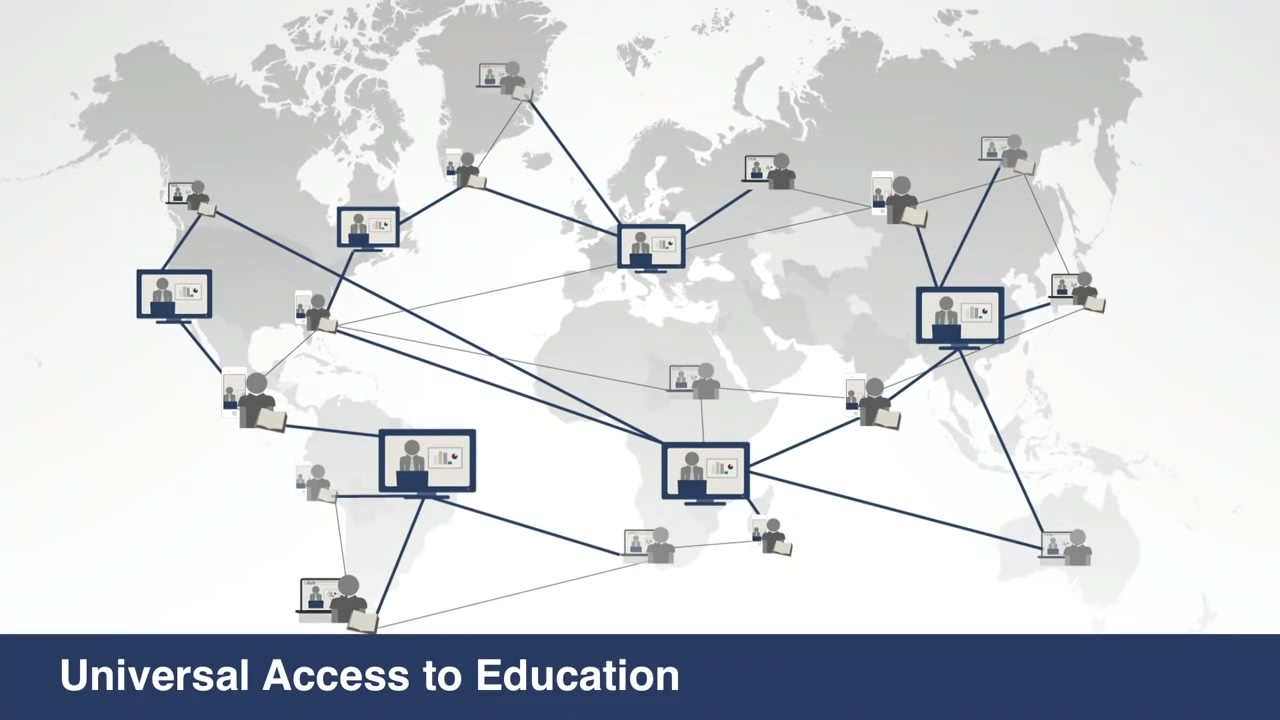
\includegraphics[width=0.8\textwidth]{world_mooc.png}%{coursera_participation.jpg}
	\end{figure}
	\vspace{-10pt}
	The expanding top-quality online education will
	\begin{itemize}
		\item Make education a fundamental human right
		\item Make lifelong learning possible
		\item Enable a wave of innovation
	\end{itemize}
\end{frame}
\note{
	(40s) So based on all of these arguments, the online education could be really promising. If high-quality education could be offered to everyone around the world for free, a lot of good things might happen.
	\vspace{10pt}
	
	{\color{blue} First, because anyone with the ability and motivation to learn can get the skills they need, it'll make education a fundamental human right.}
	\vspace{10pt}
	
	{\color{orange} Second, as people are able to learn new things every time they want, it'll make lifelong learning possible.}
	\vspace{10pt}
	
	{\color{red} And finally, because talented people always have access to high-quality education no matter where they are, they'll be able to come up with great ideas and contribute to worldwide innovation.}
}

%\begin{frame}
%	\frametitle{Grammar schools debate}
%	\begin{itemize}
%		\item Grammar schools
%		\begin{itemize}
%			\item Schools that make admissions decisions on the basis of academic ability
%			\item In contrast to comprehensive schools
%		\end{itemize}
%		\item Merits of grammar schools
%		\begin{itemize}
%			\item 
%
%		\end{itemize}
%	\end{itemize}
%\end{frame}

\begin{frame}\end{frame}

\end{spacing}
\end{document}